\documentclass[11pt, a4paper]{article}

\usepackage[british]{babel}
\usepackage{a4wide}
%\usepackage{palatino}
\usepackage{newcent}
\usepackage{graphicx}
\usepackage{fancyhdr}
\usepackage[hang,bf,footnotesize]{caption}
\usepackage{wrapfig}
\usepackage{subfigure}

\newcommand\wxMUN{wx\textsc{mun}}

\usepackage{hyperref}
\hypersetup{
    bookmarks=false,         % show bookmarks bar?
    unicode=false,          % non-Latin characters in Acrobat’s bookmarks
    pdftoolbar=true,        % show Acrobat’s toolbar?
    pdfmenubar=true,        % show Acrobat’s menu?
    pdffitwindow=false,     % window fit to page when opened
    pdfstartview={FitH},    % fits the width of the page to the window
    pdftitle={wxMUN Tutorial},    % title
    pdfauthor={Geert-Jan Besjes},     % author
    pdfsubject={wxMUN},   % subject of the document
    pdfnewwindow=true,      % links in new window
    colorlinks=false,       % false: boxed links; true: colored links
    linkcolor=red,          % color of internal links
    citecolor=green,        % color of links to bibliography
    filecolor=magenta,      % color of file links
    urlcolor=cyan           % color of external links
}


\rfoot{\setlength{\unitlength}{1mm}
 \begin{picture}(0,0)
 \put(-43,-10.35){
\includegraphics[height=12.35mm]{unllogo.png}}
 \end{picture}}
\lfoot{\setlength{\unitlength}{1mm}
 \begin{picture}(0,0)
 \put(0,-10.35){
\includegraphics[height=12.35mm]{logo.png}}
 \end{picture}}

\lhead{\textbf{\thepage}}
\rhead{\textsc{wxMUN tutorial}}
\cfoot{}

\renewcommand{\footrulewidth}{\headrulewidth}

%\addtolength{\footskip}{15mm}
\addtolength{\textheight}{0mm}

\let\oldmarginpar\marginpar
\renewcommand\marginpar[1]{\-\oldmarginpar[\raggedright\footnotesize #1]%
{\raggedleft\footnotesize #1}}

\pagestyle{fancy}
\begin{document}
\pagenumbering{roman}

\thispagestyle{empty}

\vspace*{\fill}
\vspace*{\fill}
\begin{center}
\textbf{\huge{wxMUN}}\\[1em]
\emph{\large{A Short Tutorial}}
\end{center}
\vspace*{\fill}
\vspace*{\fill}
\vspace*{\fill}
\vspace*{\fill}
\vspace*{\fill}
\hfill \emph{Draft --- \today}

\newpage
\pagenumbering{arabic} 
\setcounter{page}{1}

\section*{Introduction}
This is a short tutorial for \wxMUN , a program to manage Model United Nations (\textsc{mun}) debates. It uses the graphical toolkit wxWidgets for the user interface. The information below is current as of version 0.38 of the program. All screenshots in this document are from the same version\footnote{These screenshots are all from a Linux desktop with \textsc{kde} 3.5 as window manager -- when using either Windows or a different window manager, the interface can look slightly different.}.

\wxMUN 's homepage can be found at \url{http://wxmun.unitednetherlands.org} and is graciously hosted by \href{http://www.unitednetherlands.org}{United Netherlands}.

\section{Installing}
\wxMUN\ can be installed on a variety of platforms. Please follow the instructions for the one you are installing the program on.

\subsection{Windows}
\wxMUN\ can be installed easily: just follow the on-screen instructions in the installer. Shortcuts will automatically be placed on both your desktop and in the start menu.
\subsubsection{`Application configuration' errors}
In case you get errors relating to the `application configuration', chances are good your computer lacks Microsoft's Visual C++ Redistributable, which is required to run \wxMUN . The package is bundled with the \wxMUN\ installer and must be installed if it has never been installed before.

You can also manually install the redistributable by downloading the \emph{Microsoft Visual C++ 2008 Redistributable Package} from Microsoft's download center\footnote{\url{http://www.microsoft.com/downloads}} and following the installation instructions.

\subsection{Linux/Unix}
Currently, no binaries exist and as such you must compile \wxMUN\ from source. If you do not have any experience with this, don't worry - by following the default instructions you should be fine. 

For the highly impatient: \texttt{./configure}, \texttt{make}, (optionally) \texttt{make check} and finally (as root) \texttt{make install} should do the trick.

Prerequisites for compiling are (naturally) a working compiler, wxWidgets 2.8.x and Xerces-C++ 2.8.x. Note that you will also need to install the \emph{development versions of wxWidgets and Xerces-C++} if your system is based on installing packages (e.g. deb or rpm). Most systems are, if you are not using such a system (e.g. Gentoo, Linux From Scratch) you should know how to compile programs from source at any rate or be familiar with figuring stuff like this out anyway. Of course you will also need a copy of (\texttt{g})\texttt{make}.

Refer to your system documentation to find out how these packages are actually called and how to install them. Debian and Ubuntu users: note that wxWidgets provides installation packages for your distribution on its own homepage.

Compiling the program should now be very straightforward. The full process including all possible options is explained in \texttt{INSTALL}, also including (under `Basic Installation') the explanation how to invoke the compiler.

\subsection{MacOSX}
No (universal) binary is provided at the moment, but by installing \textsc{gcc} (the \textsc{gnu} Compiler Collection) on your system you should be able to get the application running -- wxWidgets also exists for the Mac (wxMac).

\subsection{Other}
On any other platform you can of course always try and compile \wxMUN\ from source. Note that wxWidgets and Xerces-C++ must be available in binary format or be compilable on the platform of your choice for this method to succeed.

If somehow the program still does not run, please send an email (see p. \pageref{email}).

\section{Running wxMUN}
Running \wxMUN\ should work fine now -- on Windows, double-click the executable or shortcut, on Linux/Unix type \texttt{wxmun} (or, in case you have not used \texttt{make install} or installed into a directory not included in your \texttt{PATH}, the full path of the executable) to start the program.

\begin{wrapfigure}[17]{r}{0.45\textwidth}
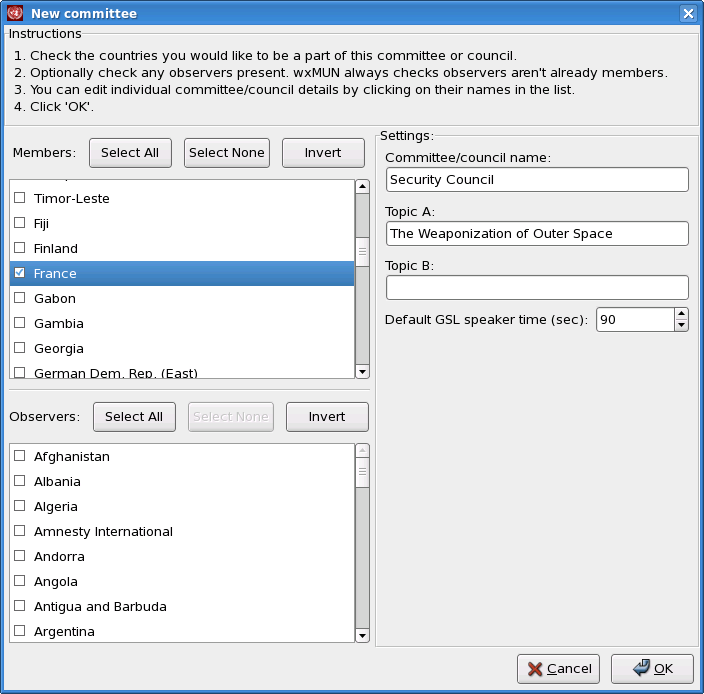
\includegraphics[width=0.45\textwidth]{screenshots/new_committee.png}
\caption{Creating a new committee, in this case a Security Council.}
\end{wrapfigure}

On startup, \wxMUN\ will check if there is a new version of the program available.

\subsection{Creating and loading a committee}
\subsubsection{Creating a new committee}
Your first order of business to be able to manage debate is to actually have something to manage: you must create a committee. This can be done through \emph{Committee $\rightarrow$ New}. 

What you see is a screen that allows you to create a new committee definition. Required for the creation are a \emph{name}, a \emph{topic} \textsc{a}, and \emph{at least one member}. Select all countries that are members and observers and simply press \textsc{ok}. The invert button can be used to invert the selection on either of the lists. \wxMUN\ will always make sure a country is only selected in one of the lists, so when inverting one list changes in the other can occur.

Next, you will be asked to save your newly created commitee somewhere. For the technically inclined reader: the committee is saved in \textsc{xml}-format.

After you have saved your committee, \wxMUN\ will ask if you wish to load it. 

\subsubsection{Loading a committee}
Committees can be loaded automatically immediately after creation, or manually through \emph{Committee $\rightarrow$ Load}.

If you are already managing another committee, keep in mind that \wxMUN\ manages \emph{one} committee at a time. If you wish to save your current state of debate, use \emph{File $\rightarrow$ Save As} to save the state as a seperate file. Again, this file simply contains \textsc{xml}.

\subsubsection{Editing a committee}
Editing a committee is done in the same way as creating one, the only difference being that the currently chosen values are already filled in. After editing a committee, you will be asked if you wish to load it or not:

\begin{itemize}
\item if you chose to load the committee without preserving the current state of debate, the effect is the same as loading the committee through \emph{Committee $\rightarrow$ Load} and the General Speakers' List will be cleared; 

\item in case you preserve the state of debate, the General Speakers' List is kept intact, but any countries no longer a member or observer will of course be removed from it;

\item if you do not load the committee, nothing happens -- you will simply have saved an extra committee definition somewhere on disk.
\end{itemize}

\subsection{Editing the database of countries}
The countries \wxMUN\ `knows about' are those contained in \texttt{countries.xml}. In the current version of \wxMUN\ you can unfortunately not edit this file through a graphical interface yet, but will have to do this manually.

Under Windows, you will find this\footnote{Note to self: the \textsc{gui} should save the file there in future when someone edits the database.} in the \texttt{data}-directory in the \texttt{share}-subdirectory, on a Linux/Unix system you will probably find it, depending on your system's configuration, in \texttt{/usr/share/wxmun} or \texttt{/usr/local/share/wxmun}.

Keep in mind the following when adding or changing a country:
\begin{enumerate}
\item its code \emph{must} be unique. In case of duplicate code entries, later entries will simply overwrite earlier ones;
\item names \emph{must} be unique;
\item the code is also used to display flags. \wxMUN\ expects flags to be in \textsc{png}-format and as such simply adds \texttt{.png} to the code 
entered. If this file does not exist, no flag is displayed at all\footnote{Note to self: figure out what happens with data that is in fact not in the right format\ldots}. Put the file in XXX\footnote{Note to self: this should not be the global data directory, but where is the user data directory exactly on Windows?} to be displayed.
\end{enumerate}

\subsection{Managing debate}
\begin{wrapfigure}[18]{l}{0.34\textwidth}
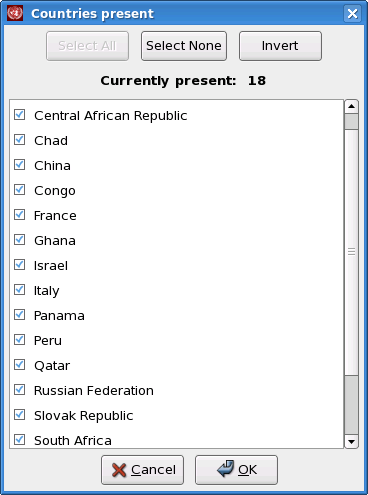
\includegraphics[width=0.34\textwidth]{screenshots/countries_present.png}
\caption{Editing the countries present.}
\end{wrapfigure}

Once you have loaded a committee, you are ready to start managing debate. The first order of business should be to find out which countries are present and tell \wxMUN\ this.
\subsubsection{Countries present}

Which countries are present in the committee at the current time can be specified through \emph{Manage debate $\rightarrow$ Countries Present}. Simply check all countries that are present and uncheck any that are (perhaps no longer) present. Indicating that countries are `present and voting' is impossible in \wxMUN , you will have to keep track of this yourself when using the Roll Call Vote tab.

Note that any country on the General Speakers' List which is indicated not to be present will \emph{not} automatically be removed. However, once any country not present is on top of the list and the next speaker is called for, \wxMUN\ will remove the country in question and continue with the next country. If that country is not present either, the process continues until the country first on the list is in fact present.

The only changes that occur when editing the list of countries present are the select-lists present throughout all tabs. Also, keep in mind that the countries present \emph{can not be edited once you enter the final voting procedure}. \wxMUN\ will remind you of this.

Finally, once countries are present, \emph{you are required to select a topic if you have multiple topics}. Any tab other than `Procedural Voting' can not be used at this time. This tab is available to allow you to have speakers in favour or against setting the agenda to a particular topic.

\subsubsection{General Speakers' List}
\begin{wrapfigure}[15]{r}{0.40\textwidth}
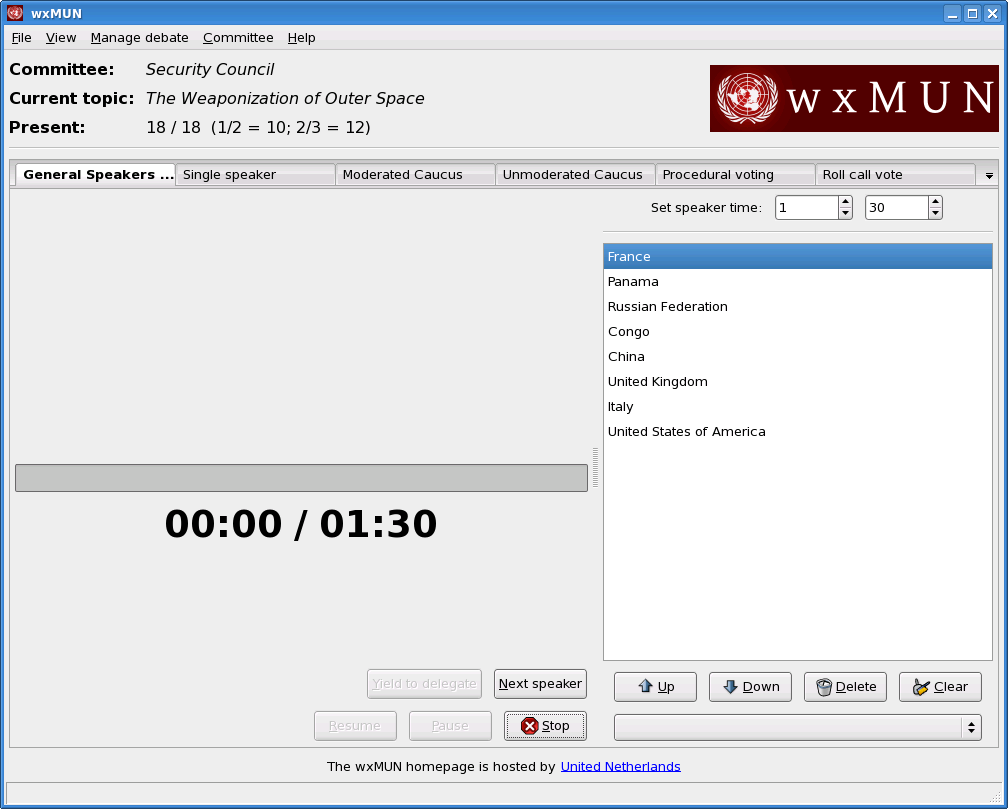
\includegraphics[width=0.40\textwidth]{screenshots/gsl.png}
\caption{The General Speakers' List.}
\end{wrapfigure}

Once there are countries present, you can draw up a General Speakers' List. Simply select the country from the drop-down list and it will be added. 

The order of the \textsc{gsl} can be edited using the `Up', `Down' and `Delete' buttons. Because of the important nature of the list, you will be asked to confirm the deletion of a country to prevent accidental removal.

Calling upon the next speaker can be done in two ways: by double-clicking the country on top of the list or by clicking the `Next Speaker' button. Double-clicking any other country than the first on the list has no effect.

The time given allotted to each speaker can be set at any time, except during speeches themselves. Simply use the indicators immediately above the list itself to change it.

Any change to the \textsc{gsl} itself or the time is automatically saved. If you restart \wxMUN\ you will return to the state the program previously was in. This state is, for Linux/Unix, saved under \texttt{\~{}/.wxmun} and for Windows in \textbf{XXX}.

\subsubsection{(Un)moderated caucus}
\begin{wrapfigure}[15]{l}{0.40\textwidth}
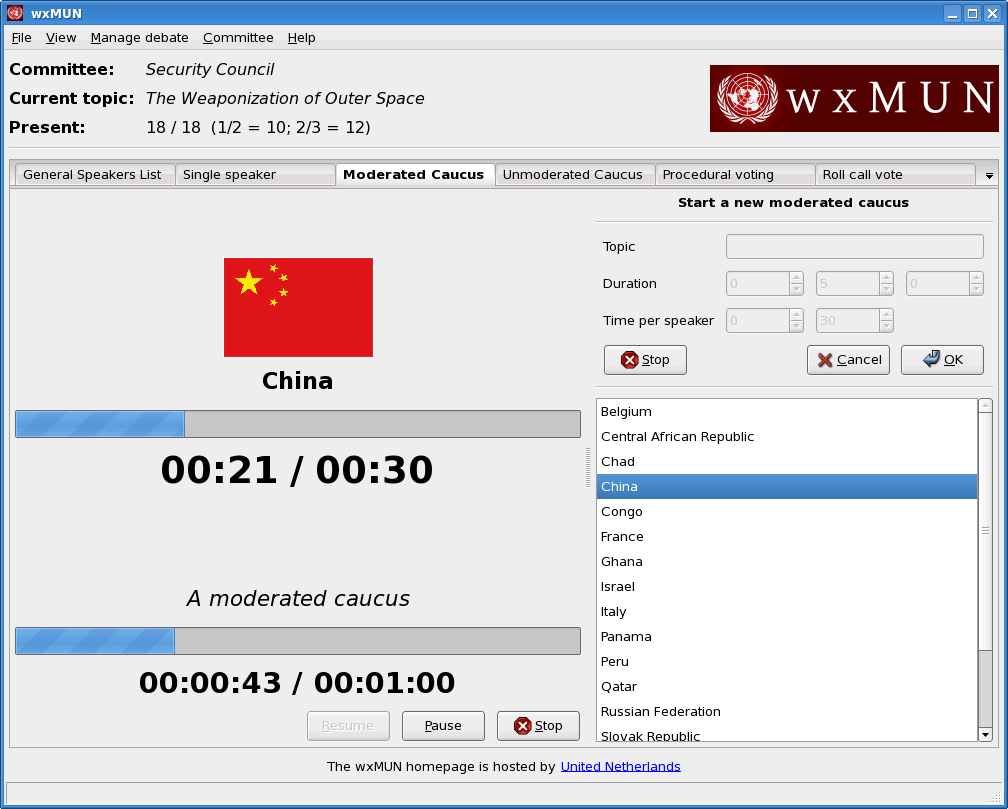
\includegraphics[width=0.40\textwidth]{screenshots/mod_caucus.png}
\caption{An example of a moderated caucus.}
\end{wrapfigure}

Starting a caucus should be extremely easy: simply use the input fields and hit OK. For an unmoderated caucus, the topic is optional. Caucuses end when the total time elapses or when you manually use `Stop'. 

When in moderated caucus, simply double-click any country name to give the floor to its delegate.

Note that for a moderated caucus, it still is allowed to call upon a speaker when the speaker time is longer than the time remaining in the caucus (e.g. 30 seconds, but there are only 8 seconds left in the caucus). This is to allow the dais to use their own personal preference in this matter, simply end the caucus manually if you do not want to allow such kind of final speakers.

\subsubsection{Procedural voting}
\begin{wrapfigure}[16]{r}{0.4\textwidth}
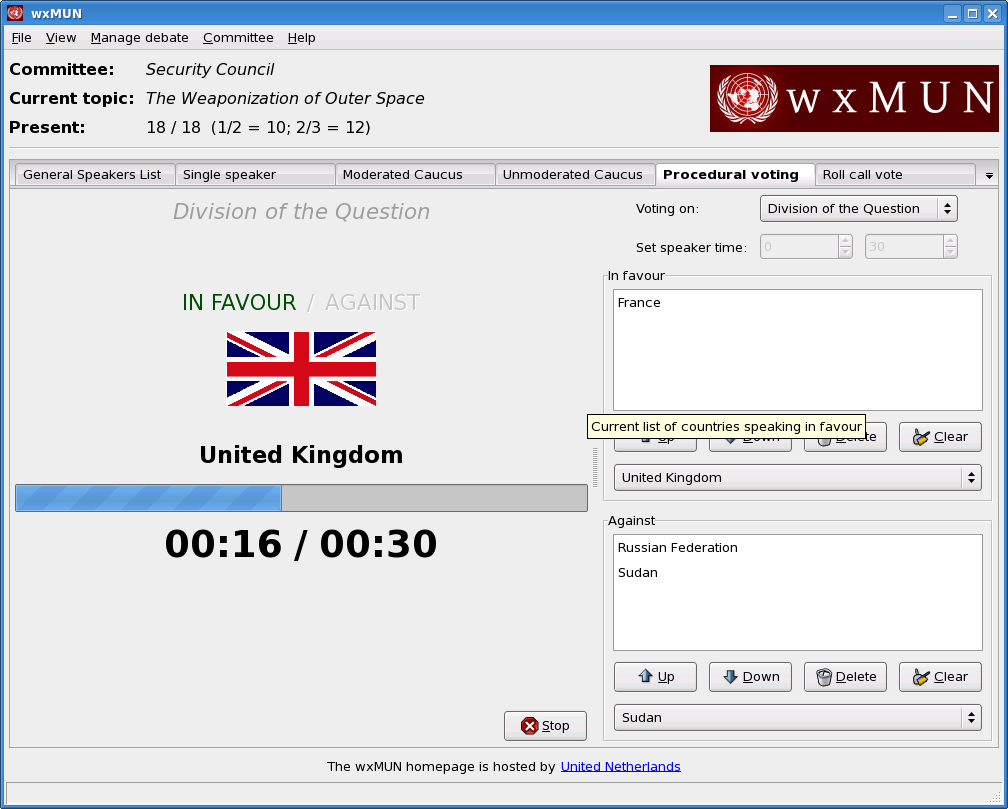
\includegraphics[width=0.4\textwidth]{screenshots/proc_voting.png}
\caption{Voting on whether or not to divide the question.}
\end{wrapfigure}

The `Procedural voting' tab can be used for anything that requires speakers in favour and against. The drop-down list only sets a label and has no other effect -- it is not required to set this label. For obvious reasons, a country cannot be both on the in favour and against lists. Selecting a country to add it to either of the lists has no effect in case it already is present on the other.

Again you can simply double-click the first country on either of the lists to give its delegate the floor. 

Note that \wxMUN\ does not force you to use the same amount of speakers in favour of a particular motion as there are against nor does it require you to alternate between the lists.

\subsubsection{Roll Call Vote}
\begin{figure}[tbp]
\centering
\subfigure[First round] % caption for subfigure a
{
    \label{fig:sub:a}
    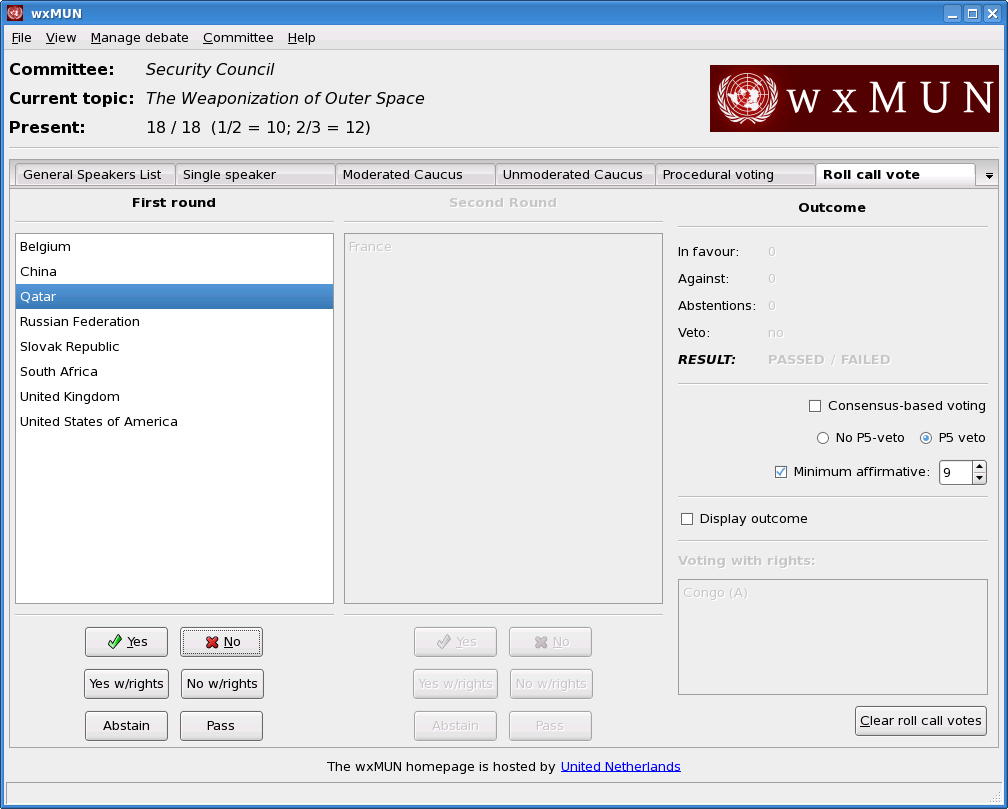
\includegraphics[width=0.315\textwidth]{screenshots/rollcall_first.png}
}
%\hspace{0.5cm}
\subfigure[Second round.] % caption for subfigure b
{
    \label{fig:sub:b}
    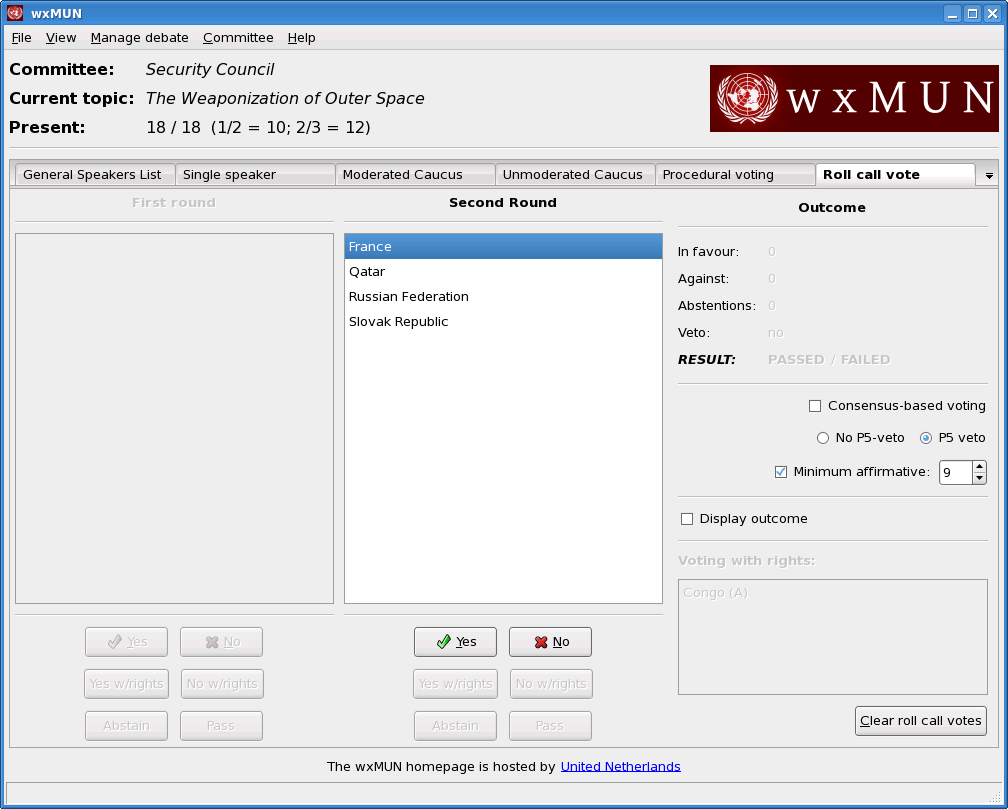
\includegraphics[width=0.315\textwidth]{screenshots/rollcall_second.png}
}
%\hspace{0.5cm}
\subfigure[Outcome.] % caption for subfigure b
{
    \label{fig:sub:c}
    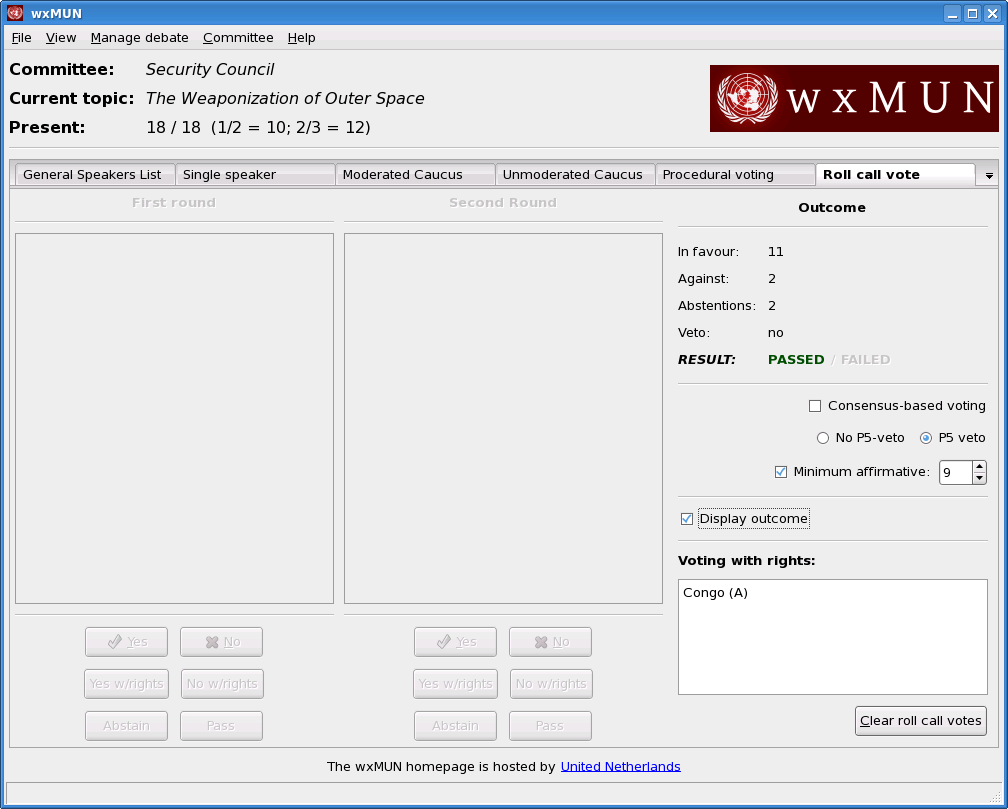
\includegraphics[width=0.315\textwidth]{screenshots/rollcall_outcome.png}
}
\caption{A roll call vote requiring the affirmative votes of the P5 and 9 votes in favour to pass. Congo has voted `no with rights'.}
\label{fig:sub} % caption for the whole figure
\end{figure}

The `Roll Call Vote' tab is unavailable until you enter voting procedure via \emph{Manage Debate $\rightarrow$ Start Voting Procedure}. Please note that it is impossible to edit the countries present once you have done this. Once you start voting procedure, any other tab can no longer be used. This is \emph{not} saved in the state of debate, so you can at any time close the program and restart it to return to the state debate was in prior to clicking on `Start Voting Procedure'.

The Roll Call Vote tab is based on the Rules of Procedure used at Harvard National Model United Nations and WorldMUN. As such, you will only find countries that are both a member of the committee or council you are simulating and are present. Any observer nation will not be shown in the lists. Again, please keep in mind that you must indicate which members are in fact present before starting a roll call vote!

In case the Rules of Procedure you are using do not contain the notion of multiple rounds, it suffices to not use the `Pass' button in the first round. This naturally equates to each country being called only once. 

The `with rights' buttons only differ from the normal ones in that they add countries to the list in the right-hand corner which you can, after the vote has concluded, double-click to allow explanations of votes against country policy if your Rules of Procedure allow this. \wxMUN\ will automatically switch to the Single Speaker tab to display the time.

To actually proceed in taking a vote, simply use the first round list starting from the member you randomly chose and use the buttons below the list. \wxMUN\ will always cycle to the next country on the list for convenience. Once the first list is exhausted, the list for the second round becomes available if there are any countries that passed during the first round. If this is the case, proceed with the second round until that list is empty as well.

Once you are done taking the vote, select `Display outcome' to show the outcome. By default, \wxMUN\ calculates whether the vote has passed by requiring a simple majority: if there are more countries voting `yes' than `no', the outcome is a pass.

You can deviate from this default setting in multiple ways:

\begin{description}
\item[Consensus-based voting.] If you check this box, any vote against will cause the document you are voting on to fail;
\item[P5-veto.] If any of the permanent members of the Security Council voted against, the vote fails. Note that \wxMUN\ uses the composition of the \textsc{sc} since 1991 to determine if a country is a permanent member, it is currently impossible\footnote{Note to self: this is downright stupid.} to use this option with either the Soviet Union, the Republic of China or both;
\item[Mininum affirmative.] If the vote requires a different majority than a simple majority you can specify the required number of votes in favour. If this threshold is then exceeded, the document voted upon passes. Note that this is for example required for a Security Council simulation, where 9 votes in favour (instead of a simple majority of countries voting) are always needed.
\end{description}
The last two options can of course be combined. Also, it is worthwile to remember that these options can all be changed at any time, including \emph{before} displaying the outcome.

Finally, please note again that \wxMUN\ has \emph{no notion} of the concept `present and voting'. You must remember yourself whether countries are allowed to abstain or not.

\section{Bugs and questions}
In case you find a bug in \wxMUN\, we urge you to please send us an email. This helps to improve the experience for other users. Also, if you feel a certain feature could be added to the program, do not hesitate to ask. 

Finally, especially if anything is unclear regarding either this document or \wxMUN\ itself, drop a note!

\vfill
\noindent 
Geert-Jan Besjes, \texttt{g.besjes@student.science.ru.nl} \label{email} \\
\emph{Last compiled: \today}

\end{document}
